\documentclass{article}
\usepackage{tikz}
\usepackage{amsmath}
\usetikzlibrary{matrix}
\title{Connect 4 AI}
\author{David Friedman \and Sridatt Bhamidipati}


\tikzstyle{player} = [circle, minimum size=.4cm, draw=black]
\tikzstyle{threat} = [rectangle, thick, minimum size=.4cm, draw=blue]

\usepackage{subcaption} 
\usepackage{cleveref}

\newcommand{\rd}{\node [player, fill=red]{};}
\newcommand{\yw}{\node [player, fill=yellow] {};}
\newcommand{\gy}{\node [player, fill=white] {};}
\newcommand{\rt}{\node [threat, fill=red!50] {};}
\newcommand{\yt}{\node [threat, fill=yellow!50] {};}
\newcommand{\bt}{\node [threat, fill=orange!50] {};}



\begin{document}
	\maketitle
	\newpage
	\tableofcontents
	\newpage
	
	\section{Evaluation}
		\subsection{Functions}
		Our evaluation function is a combination of two evaluation functions.
		\subsubsection{Number owned in winning group}
		Our first evaluation function is a a count of all winning groups we own, weighted by the number we own in that group minus the count of all winning groups the opponent owns, again weighted by the number they own in that group. The equation for this is:
		\[f_1(x)=\sum_{n \in s_{1,r}}{numOwned_1(n)}-\sum_{n \in s_{2,r}}{numOwned_2(n)}\]
		where $numOwned_{r,n}$ represents the number owned by player $r$ in the winning group n, and $s_r$ represents the winning groups soley owned by player $r$.
		\subsubsection{Odd/Even Threats}
		Our second evaluation function is more complicated. First it iterates over a list of all possible winning groups, and finds the threats. A threat is a slot that would complete a 4 in a row for either team. It then iterates over each of these threats and tallies them, categorizing them based on the teamwho owns the threat and the threats polarity. Even threats are threats that have an even number of (necessarily) empty spaces above them, while odd are threats with an odd number of empty spaces above them (figure \ref{threattypes}). The function ignores a threat if there is a threat below it from the opposite team with opposite polarity (the reasoning will be explained in the section \ref{ssec:reasoning}). 
		
		The function then checks if player 1 has more odd threats than player 2, if player 2 has two more odd threats than player one, or, if in the case they both have the same number, if player 2 has at least one even threat. If the former is satisfied it returns $100$, signifying that player one is in the lead. For the former two it returns $-100$, signifying the opposite, and if none of the cases are satisfied we return 0. The equation looks like the following piecewise:
		\[ f_2(x,y)=\begin{cases} 
		      100 & odd(x)>odd(y) \\
		     -100 & odd(y)>odd(x)+1 \\
		     -100 & odd(x)=odd(y)~\mbox{and}~even(y) > 0\\
		      0 & otherwise
		   \end{cases}
		\]
where x is all threats by player 1, and y is all threats by player 2.
		
		\begin{figure}[t]
		\centering
			\begin{subfigure}[b]{0.4\textwidth}
			\centering
			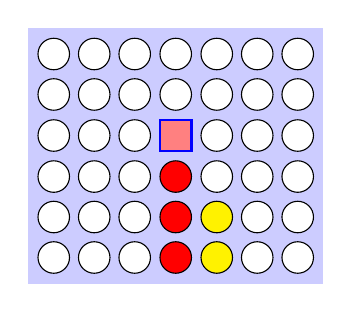
\begin{tikzpicture}
				\fill[blue!20] (0,0) rectangle (3.75,3.25);
				\matrix (mat) at (0,0) [matrix of nodes, ampersand replacement=\&, nodes={circle, minimum size=.4cm},
				anchor= south west,
				column sep={.1cm}, row sep={.1cm}] {
					\gy \& \gy \& \gy \& \gy \& \gy \& \gy \& \gy \\
					\gy \& \gy \& \gy \& \gy \& \gy \& \gy \& \gy \\
					\gy \& \gy \& \gy \& \rt \& \gy \& \gy \& \gy \\
					\gy \& \gy \& \gy \& \rd \& \gy \& \gy \& \gy \\
					\gy \& \gy \& \gy \& \rd \& \yw \& \gy \& \gy \\
					\gy \& \gy \& \gy \& \rd \& \yw \& \gy \& \gy \\
				};
			\end{tikzpicture}
			\caption{Even red threat}
			\label{threatodd}
			\end{subfigure}%
			\begin{subfigure}[b]{0.4\textwidth}
			\centering
			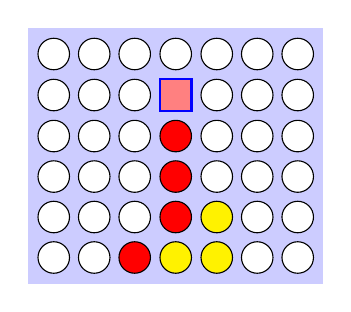
\begin{tikzpicture}
				\fill[blue!20] (0,0) rectangle (3.75,3.25);
				\matrix (mat) at (0,0) [matrix of nodes, ampersand replacement=\&, nodes={circle, minimum size=.4cm},
				anchor= south west,
				column sep={.1cm}, row sep={.1cm}] {
					\gy \& \gy \& \gy \& \gy \& \gy \& \gy \& \gy \\
					\gy \& \gy \& \gy \& \rt \& \gy \& \gy \& \gy \\
					\gy \& \gy \& \gy \& \rd \& \gy \& \gy \& \gy \\
					\gy \& \gy \& \gy \& \rd \& \gy \& \gy \& \gy \\
					\gy \& \gy \& \gy \& \rd \& \yw \& \gy \& \gy \\
					\gy \& \gy \& \rd \& \yw \& \yw \& \gy \& \gy \\
				};
			\end{tikzpicture}
			\caption{Odd red threat}
			\label{threateven}
			\end{subfigure}%
			\caption{Types of threats (threat marked with squares)}
			\label{threattypes}
		\end{figure}
		\subsection{Reasoning}
		\label{ssec:reasoning}
		Our first evaluation function is straightforward. We want to value states where we have more control of the winning positions more. If we control a winning position (only our pieces are in it), we can use it to win. If the enemy controls it they can use it to win. Additionally, if more of our/their pieces are in a winning position, we need less moves to complete that win, which is favourable.
		
		Our second evaluation function is more complicated. It relies on the fact that red (player 1) will only ever move when there are an even number of pieces on the board, and yellow (player 2) will only ever move when there are an odd number of pieces on the board. Additionally it relies on the fact that since columns have an even number of slots, red generally has more control over odd positions than even (as if a column is completely full, red still may move in the bottom odd column). This means red has an easier time taking odd threats, and yellow has an easier time taking even threats. Therefore, it is logical that red can generally block all of yellows threats and grab its own winning attack if it has more of these odd threats. Yellow on the other hand needs to have two more odd threats, as if it only has one more red may use its advantage in playing odd rows to block all these attacks before yellow can win. The last case is because if they have an equal number of threats, once red has blocked all of yellows odd threats, yellow will generally have an easier time grabbing an even row, and thus winning with its even attack.
		
		It needs to be explained \emph{why} we remove threats above another threat if the threat is from the other player and has a different parity. This is quite simple. Take figure \ref{threatblock} as an example. Here orange squares represent threats both players own. Note that yellow has an even threat here. However, in order to take it the slot beneath must be filled. Because there are an even number of pieces played (each column is an even number high), it is reds turn. Red has an odd threat in the first row. Therefore yellows threat may never be taken, as red must play below first and win. If we for now ignore all but yellows first even threat and reds even threat above it, we can see that the same thing would occur. Therefore in general threats of opposite parity to lower threats by the other player are useless. We can extend this to also mark shared threats by yellow on odd levels as useless for yellow, and shared even threats as useless for red, but we leave this out of our code for simplicity.
		
			\begin{figure}[t]
			\centering
			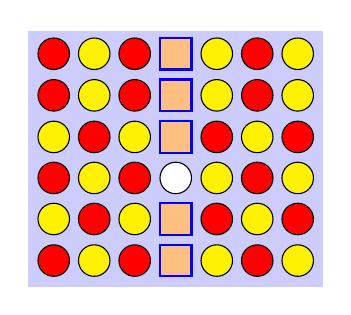
\begin{tikzpicture}
				\fill[blue!20] (0,0) rectangle (3.75,3.25);
				\matrix (mat) at (0,0) [matrix of nodes, ampersand replacement=\&, nodes={circle, minimum size=.4cm},
				anchor= south west,
				column sep={.1cm}, row sep={.1cm}] {
					\rd \& \yw \& \rd \& \bt \& \yw \& \rd \& \yw \\
					\rd \& \yw \& \rd \& \bt \& \yw \& \rd \& \yw \\
					\yw \& \rd \& \yw \& \bt \& \rd \& \yw \& \rd \\
					\rd \& \yw \& \rd \& \gy \& \yw \& \rd \& \yw\ \\
					\yw \& \rd \& \yw \& \bt \& \rd \& \yw \& \rd \\
					\rd \& \yw \& \rd \& \bt \& \yw \& \rd \& \yw \\
				};
			\end{tikzpicture}
			\caption{Useless yellow threat}
			\label{threatblock}
			\end{figure}
	\subsection{Worked Example}
	We will use figure \ref{fig:example} as our example game state. First we will run our second heuristic, as it is much simpler to run in this case. Threats have been marked their respective team colors. Red has two odd threats, and yellow has one even threat. This means we have $odd(x) > odd(y)$, and our evaluation function returns 100.
	
	Our second heuristic is a bit lengthier to run through, as there are a total of 69 winning positions we need to consider. However, here only 8 are winning positions that are not invalid due to having two different players in them, and two of those (the rightmost column starting from the top and the second highest down) have no pieces in them. We can easily count the number owned by red and yellow, and we see that the result is $7-6 = 1$, which again is favourful to red. As seen in figure \ref{fig:win}, this is correct and red does win.
			\begin{figure}[t]
			\centering
			\begin{subfigure}[b]{0.4\textwidth}
				\centering
				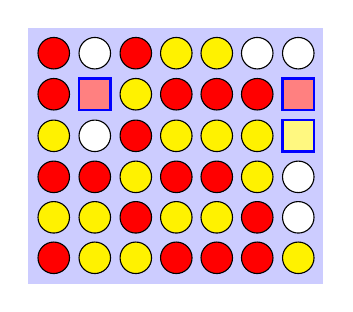
\begin{tikzpicture}
					\fill[blue!20] (0,0) rectangle (3.75,3.25);
					\matrix (mat) at (0,0) [matrix of nodes, ampersand replacement=\&, nodes={circle, minimum size=.4cm},
					anchor= south west,
					column sep={.1cm}, row sep={.1cm}] {
						\rd \& \gy \& \rd \& \yw \& \yw \& \gy \& \gy \\
						\rd \& \rt \& \yw \& \rd \& \rd \& \rd \& \rt \\
						\yw \& \gy \& \rd \& \yw \& \yw \& \yw \& \yt \\
						\rd \& \rd \& \yw \& \rd \& \rd \& \yw \& \gy \\
						\yw \& \yw \& \rd \& \yw \& \yw \& \rd \& \gy \\
						\rd \& \yw \& \yw \& \rd \& \rd \& \rd \& \yw \\
					};
				\end{tikzpicture}
				\caption{Red to win}
				\label{fig:example}
			\end{subfigure}
			\begin{subfigure}[b]{0.4\textwidth}
				\centering
				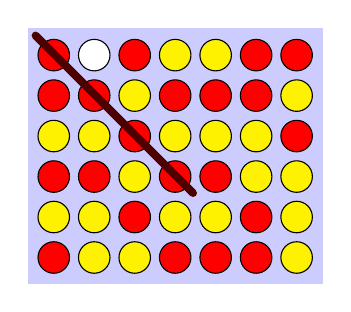
\begin{tikzpicture}
					\fill[blue!20] (0,0) rectangle (3.75,3.25);
					\matrix (mat) at (0,0) [matrix of nodes, ampersand replacement=\&, nodes={circle, minimum size=.4cm},
					anchor= south west,
					column sep={.1cm}, row sep={.1cm}] {
						\rd \& \gy \& \rd \& \yw \& \yw \& \rd \& \rd \\
						\rd \& \rd \& \yw \& \rd \& \rd \& \rd \& \yw \\
						\yw \& \yw \& \rd \& \yw \& \yw \& \yw \& \rd \\
						\rd \& \rd \& \yw \& \rd \& \rd \& \yw \& \yw \\
						\yw \& \yw \& \rd \& \yw \& \yw \& \rd \& \yw \\
						\rd \& \yw \& \yw \& \rd \& \rd \& \rd \& \yw \\
					};
					\draw[line width=.1cm, draw=red!30!black, cap=round] (.1,3.15) -- (2.1, 1.15);
				\end{tikzpicture}
				\caption{Red wins}
				\label{fig:win}
			\end{subfigure}
			\caption{Example}
			\end{figure}
	\newpage
	\section{MiniMax Against poor AI}
	\subsection{Against StupidAI}
	\begin{figure}[h]
	\centering
	\begin{subfigure}[b]{0.4\textwidth}
	\centering
	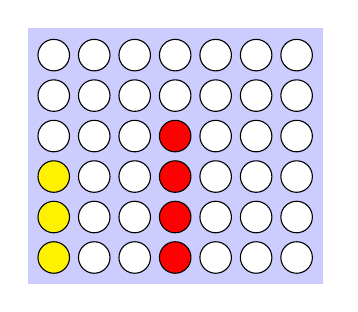
\begin{tikzpicture}
				\fill[blue!20] (0,0) rectangle (3.75,3.25);
				\matrix (mat) at (0,0) [matrix of nodes, ampersand replacement=\&, nodes={circle, minimum size=.4cm},
				anchor= south west,
				column sep={.1cm}, row sep={.1cm}] {
					\gy \& \gy \& \gy \& \gy \& \gy \& \gy \& \gy \& \\
					\gy \& \gy \& \gy \& \gy \& \gy \& \gy \& \gy \& \\
					\gy \& \gy \& \gy \& \rd \& \gy \& \gy \& \gy \& \\
					\yw \& \gy \& \gy \& \rd \& \gy \& \gy \& \gy \& \\
					\yw \& \gy \& \gy \& \rd \& \gy \& \gy \& \gy \& \\
					\yw \& \gy \& \gy \& \rd \& \gy \& \gy \& \gy \& \\
				};
	\end{tikzpicture}
	\caption{As player 1}
	\label{fig:stup1}
	\end{subfigure}
	\begin{subfigure}[b]{0.4\textwidth}
	\centering
	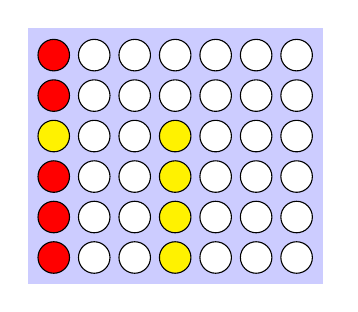
\begin{tikzpicture}
				\fill[blue!20] (0,0) rectangle (3.75,3.25);
				\matrix (mat) at (0,0) [matrix of nodes, ampersand replacement=\&, nodes={circle, minimum size=.4cm},
				anchor= south west,
				column sep={.1cm}, row sep={.1cm}] {
					 \rd \& \gy \& \gy \& \gy \& \gy \& \gy \& \gy \& \\
					 \rd \& \gy \& \gy \& \gy \& \gy \& \gy \& \gy \& \\
					 \yw \& \gy \& \gy \&  \yw \& \gy \& \gy \& \gy \& \\
					 \rd \& \gy \& \gy \&  \yw \& \gy \& \gy \& \gy \& \\
					 \rd \& \gy \& \gy \&  \yw \& \gy \& \gy \& \gy \& \\
					 \rd \& \gy \& \gy \&  \yw \& \gy \& \gy \& \gy \& \\
				};
	\end{tikzpicture}
	\caption{As player 2}
	\label{fig:stup2}
	\end{subfigure}
	\end{figure}
	
	If MiniMax goes first see \ref{fig:stup1} otherwise see \ref{fig:stup2}. Games depend only on who goes first (we use no randomness so seed has no effect).
	
	\newpage
	\subsection{Against RandomAI}
	
	\begin{figure}[h]
		\centering
\begin{subfigure}[b]{0.4\linewidth}%
	\centering%
	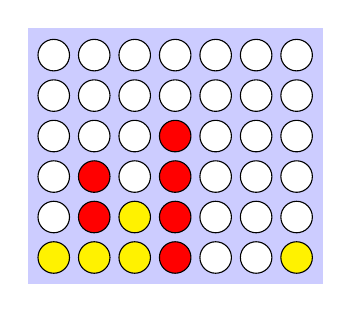
\begin{tikzpicture}%
				\fill[blue!20] (0,0) rectangle (3.75,3.25);
				\matrix (mat) at (0,0) [matrix of nodes, ampersand replacement=\&, nodes={circle, minimum size=.4cm},
				anchor= south west,
				column sep={.1cm}, row sep={.1cm}] { \gy \&  \gy \&  \gy \&  \gy \&  \gy \&  \gy \&  \gy \&  \\
	 \gy \&  \gy \&  \gy \&  \gy \&  \gy \&  \gy \&  \gy \&  \\
	 \gy \&  \gy \&  \gy \&  \rd \&  \gy \&  \gy \&  \gy \&  \\
	 \gy \&  \rd \&  \gy \&  \rd \&  \gy \&  \gy \&  \gy \&  \\
	 \gy \&  \rd \&  \yw \& \rd \&  \gy \&  \gy \&  \gy \&  \\
	 \yw \& \yw \& \yw \& \rd \&  \gy \&  \gy \&  \yw \& \\
					};
	\end{tikzpicture}%
	\caption{As player 1}%
	\label{fig:ran2}%
	\end{subfigure}%
	
	\begin{subfigure}[b]{0.4\linewidth}%
	\centering%
	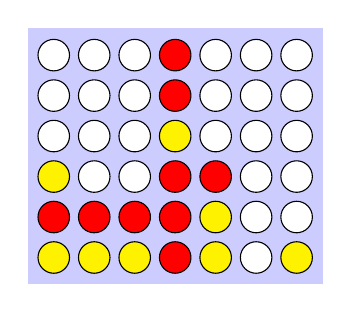
\begin{tikzpicture}%
				\fill[blue!20] (0,0) rectangle (3.75,3.25);
				\matrix (mat) at (0,0) [matrix of nodes, ampersand replacement=\&, nodes={circle, minimum size=.4cm},
				anchor= south west,
				column sep={.1cm}, row sep={.1cm}] { \gy \&  \gy \&  \gy \&  \rd \&  \gy \&  \gy \&  \gy \&  \\
	 \gy \&  \gy \&  \gy \&  \rd \&  \gy \&  \gy \&  \gy \&  \\
	 \gy \&  \gy \&  \gy \&  \yw \& \gy \&  \gy \&  \gy \&  \\
	 \yw \& \gy \&  \gy \&  \rd \&  \rd \&  \gy \&  \gy \&  \\
	 \rd \&  \rd \&  \rd \&  \rd \&  \yw \& \gy \&  \gy \&  \\
	 \yw \& \yw \& \yw \& \rd \&  \yw \& \gy \&  \yw \& \\
					};
	\end{tikzpicture}%
	\caption{As player 1}%
	\label{fig:ran2}%
	\end{subfigure}%
	%
	\begin{subfigure}[b]{0.4\linewidth}%
	\centering%
	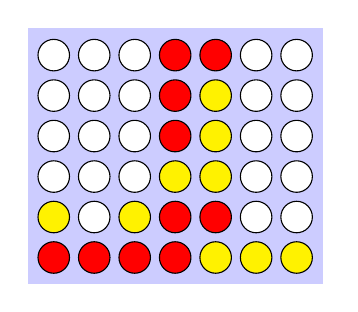
\begin{tikzpicture}%
				\fill[blue!20] (0,0) rectangle (3.75,3.25);
				\matrix (mat) at (0,0) [matrix of nodes, ampersand replacement=\&, nodes={circle, minimum size=.4cm},
				anchor= south west,
				column sep={.1cm}, row sep={.1cm}] { \gy \&  \gy \&  \gy \&  \rd \&  \rd \&  \gy \&  \gy \&  \\
	 \gy \&  \gy \&  \gy \&  \rd \&  \yw \& \gy \&  \gy \&  \\
	 \gy \&  \gy \&  \gy \&  \rd \&  \yw \& \gy \&  \gy \&  \\
	 \gy \&  \gy \&  \gy \&  \yw \& \yw \& \gy \&  \gy \&  \\
	 \yw \& \gy \&  \yw \& \rd \&  \rd \&  \gy \&  \gy \&  \\
	 \rd \&  \rd \&  \rd \&  \rd \&  \yw \& \yw \& \yw \& \\
					};
	\end{tikzpicture}%
	\caption{As player 1}%
	\label{fig:ran2}%
	\end{subfigure}%
	%
		\end{figure}%
	\begin{figure}[h]%
	\centering%
	%
	%
		\begin{subfigure}[b]{0.4\linewidth}%
	\centering%
	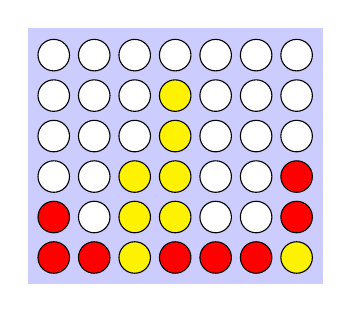
\begin{tikzpicture}%
				\fill[blue!20] (0,0) rectangle (3.75,3.25);
				\matrix (mat) at (0,0) [matrix of nodes, ampersand replacement=\&, nodes={circle, minimum size=.4cm},
				anchor= south west,
				column sep={.1cm}, row sep={.1cm}] { \gy \&  \gy \&  \gy \&  \gy \&  \gy \&  \gy \&  \gy \&  \\
	 \gy \&  \gy \&  \gy \&  \yw \& \gy \&  \gy \&  \gy \&  \\
	 \gy \&  \gy \&  \gy \&  \yw \& \gy \&  \gy \&  \gy \&  \\
	 \gy \&  \gy \&  \yw \& \yw \& \gy \&  \gy \&  \rd \&  \\
	 \rd \&  \gy \&  \yw \& \yw \& \gy \&  \gy \&  \rd \&  \\
	 \rd \&  \rd \&  \yw \& \rd \&  \rd \&  \rd \&  \yw \& \\
					};
	\end{tikzpicture}%
	\caption{As player 2}%
	\label{fig:ran2}%
	\end{subfigure}%
	%
	\begin{subfigure}[b]{0.4\linewidth}%
	\centering%
	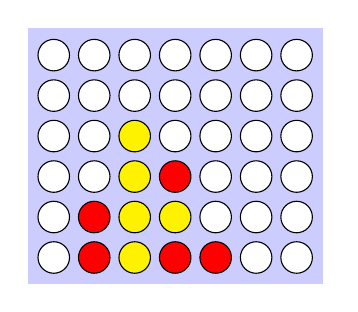
\begin{tikzpicture}%
				\fill[blue!20] (0,0) rectangle (3.75,3.25);
				\matrix (mat) at (0,0) [matrix of nodes, ampersand replacement=\&, nodes={circle, minimum size=.4cm},
				anchor= south west,
				column sep={.1cm}, row sep={.1cm}] { \gy \&  \gy \&  \gy \&  \gy \&  \gy \&  \gy \&  \gy \&  \\
	 \gy \&  \gy \&  \gy \&  \gy \&  \gy \&  \gy \&  \gy \&  \\
	 \gy \&  \gy \&  \yw \& \gy \&  \gy \&  \gy \&  \gy \&  \\
	 \gy \&  \gy \&  \yw \& \rd \&  \gy \&  \gy \&  \gy \&  \\
	 \gy \&  \rd \&  \yw \& \yw \& \gy \&  \gy \&  \gy \&  \\
	 \gy \&  \rd \&  \yw \& \rd \&  \rd \&  \gy \&  \gy \&  \\
					};
	\end{tikzpicture}%
	\caption{As player 2}%
	\label{fig:ran2}%
	\end{subfigure}%
	%
	\end{figure}%
%
%
	\newpage
	\subsection{Against MonteCarloAI}
	\newpage
	
		\begin{figure}[h]%
		\centering
	\begin{subfigure}[b]{0.4\linewidth}%
	\centering%
	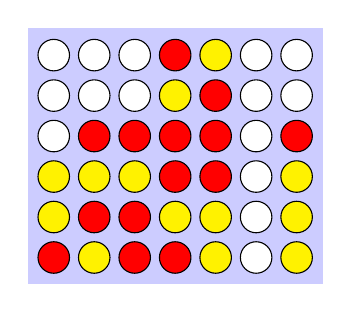
\begin{tikzpicture}%
				\fill[blue!20] (0,0) rectangle (3.75,3.25);%
				\matrix (mat) at (0,0) [matrix of nodes, ampersand replacement=\&, nodes={circle, minimum size=.4cm},%
				anchor= south west,%
				column sep={.1cm}, row sep={.1cm}] { \gy \&  \gy \&  \gy \&  \rd \&  \yw \& \gy \&  \gy \&  \\%
	 \gy \&  \gy \&  \gy \&  \yw \& \rd \&  \gy \&  \gy \&  \\%
	 \gy \&  \rd \&  \rd \&  \rd \&  \rd \&  \gy \&  \rd \&  \\%
	 \yw \& \yw \& \yw \& \rd \&  \rd \&  \gy \&  \yw \& \\%
	 \yw \& \rd \&  \rd \&  \yw \& \yw \& \gy \&  \yw \& \\%
	 \rd \&  \yw \& \rd \&  \rd \&  \yw \& \gy \&  \yw \& \\%
					};%
	\end{tikzpicture}%
	\caption{As player 1}%
	\label{fig:monty}%
	\end{subfigure}%
	%
	\begin{subfigure}[b]{0.4\linewidth}%
	\centering%
	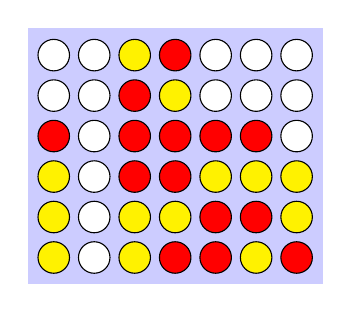
\begin{tikzpicture}%
				\fill[blue!20] (0,0) rectangle (3.75,3.25);%
				\matrix (mat) at (0,0) [matrix of nodes, ampersand replacement=\&, nodes={circle, minimum size=.4cm},%
				anchor= south west,%
				column sep={.1cm}, row sep={.1cm}] { \gy \&  \gy \&  \yw \& \rd \&  \gy \&  \gy \&  \gy \&  \\%
	 \gy \&  \gy \&  \rd \&  \yw \& \gy \&  \gy \&  \gy \&  \\%
	 \rd \&  \gy \&  \rd \&  \rd \&  \rd \&  \rd \&  \gy \&  \\%
	 \yw \& \gy \&  \rd \&  \rd \&  \yw \& \yw \& \yw \& \\%
	 \yw \& \gy \&  \yw \& \yw \& \rd \&  \rd \&  \yw \& \\%
	 \yw \& \gy \&  \yw \& \rd \&  \rd \&  \yw \& \rd \&  \\%
					};%
	\end{tikzpicture}%
	\caption{As player 1}%
	\label{fig:monty}%
	\end{subfigure}%
	
	\end{figure}
	\begin{figure}[h]
	\centering
	%
	\begin{subfigure}[b]{0.4\linewidth}%
	\centering%
	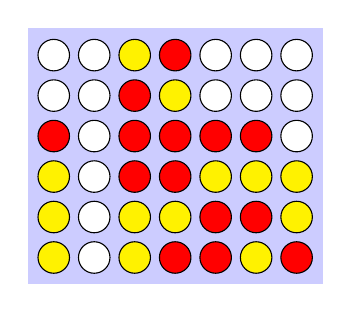
\begin{tikzpicture}%
				\fill[blue!20] (0,0) rectangle (3.75,3.25);%
				\matrix (mat) at (0,0) [matrix of nodes, ampersand replacement=\&, nodes={circle, minimum size=.4cm},%
				anchor= south west,%
				column sep={.1cm}, row sep={.1cm}] { \gy \&  \gy \&  \yw \& \rd \&  \gy \&  \gy \&  \gy \&  \\%
	 \gy \&  \gy \&  \rd \&  \yw \& \gy \&  \gy \&  \gy \&  \\%
	 \rd \&  \gy \&  \rd \&  \rd \&  \rd \&  \rd \&  \gy \&  \\%
	 \yw \& \gy \&  \rd \&  \rd \&  \yw \& \yw \& \yw \& \\%
	 \yw \& \gy \&  \yw \& \yw \& \rd \&  \rd \&  \yw \& \\%
	 \yw \& \gy \&  \yw \& \rd \&  \rd \&  \yw \& \rd \&  \\%
					};%
	\end{tikzpicture}%
	\caption{As player 1}%
	\label{fig:monty}%
	\end{subfigure}%
	%
	%
	\begin{subfigure}[b]{0.4\linewidth}%
	\centering%
	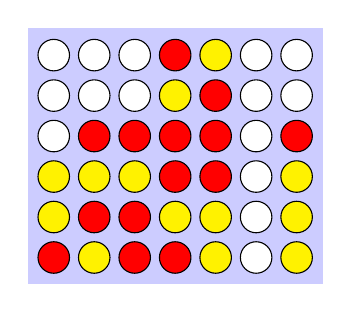
\begin{tikzpicture}%
				\fill[blue!20] (0,0) rectangle (3.75,3.25);%
				\matrix (mat) at (0,0) [matrix of nodes, ampersand replacement=\&, nodes={circle, minimum size=.4cm},%
				anchor= south west,%
				column sep={.1cm}, row sep={.1cm}] { \gy \&  \gy \&  \gy \&  \rd \&  \yw \& \gy \&  \gy \&  \\%
	 \gy \&  \gy \&  \gy \&  \yw \& \rd \&  \gy \&  \gy \&  \\%
	 \gy \&  \rd \&  \rd \&  \rd \&  \rd \&  \gy \&  \rd \&  \\%
	 \yw \& \yw \& \yw \& \rd \&  \rd \&  \gy \&  \yw \& \\%
	 \yw \& \rd \&  \rd \&  \yw \& \yw \& \gy \&  \yw \& \\%
	 \rd \&  \yw \& \rd \&  \rd \&  \yw \& \gy \&  \yw \& \\%
					};%
	\end{tikzpicture}%
	\caption{As player 1}%
	\label{fig:monty}%
	\end{subfigure}%
	
	
	\end{figure}
	\begin{figure}[h]
		\centering
	%
	\begin{subfigure}[b]{0.4\linewidth}%
	\centering%
	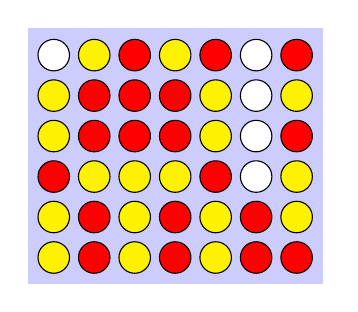
\begin{tikzpicture}%
				\fill[blue!20] (0,0) rectangle (3.75,3.25);%
				\matrix (mat) at (0,0) [matrix of nodes, ampersand replacement=\&, nodes={circle, minimum size=.4cm},%
				anchor= south west,%
				column sep={.1cm}, row sep={.1cm}] { \gy \&  \yw \& \rd \&  \yw \& \rd \&  \gy \&  \rd \&  \\%
	 \yw \& \rd \&  \rd \&  \rd \&  \yw \& \gy \&  \yw \& \\%
	 \yw \& \rd \&  \rd \&  \rd \&  \yw \& \gy \&  \rd \&  \\%
	 \rd \&  \yw \& \yw \& \yw \& \rd \&  \gy \&  \yw \& \\%
	 \yw \& \rd \&  \yw \& \rd \&  \yw \& \rd \&  \yw \& \\%
	 \yw \& \rd \&  \yw \& \rd \&  \yw \& \rd \&  \rd \&  \\%
					};%
	\end{tikzpicture}%
	\caption{As player 1}%
	\label{fig:monty}%
	\end{subfigure}%
	%
	\begin{subfigure}[b]{0.4\linewidth}%
	\centering%
	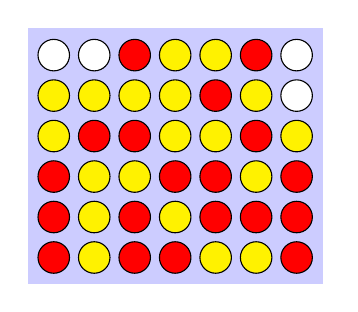
\begin{tikzpicture}%
				\fill[blue!20] (0,0) rectangle (3.75,3.25);%
				\matrix (mat) at (0,0) [matrix of nodes, ampersand replacement=\&, nodes={circle, minimum size=.4cm},%
				anchor= south west,%
				column sep={.1cm}, row sep={.1cm}] { \gy \&  \gy \&  \rd \&  \yw \& \yw \& \rd \&  \gy \&  \\%
	 \yw \& \yw \& \yw \& \yw \& \rd \&  \yw \& \gy \&  \\%
	 \yw \& \rd \&  \rd \&  \yw \& \yw \& \rd \&  \yw \& \\%
	 \rd \&  \yw \& \yw \& \rd \&  \rd \&  \yw \& \rd \&  \\%
	 \rd \&  \yw \& \rd \&  \yw \& \rd \&  \rd \&  \rd \&  \\%
	 \rd \&  \yw \& \rd \&  \rd \&  \yw \& \yw \& \rd \&  \\%
					};%
	\end{tikzpicture}%
	\caption{As player 2}%
	\label{fig:monty}%
	\end{subfigure}%
	%
	
	\end{figure}
	\begin{figure}[h]
		\centering
	
	\begin{subfigure}[b]{0.4\linewidth}%
	\centering%
	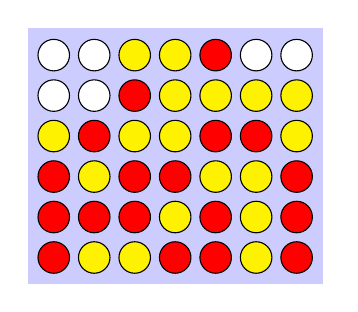
\begin{tikzpicture}%
				\fill[blue!20] (0,0) rectangle (3.75,3.25);%
				\matrix (mat) at (0,0) [matrix of nodes, ampersand replacement=\&, nodes={circle, minimum size=.4cm},%
				anchor= south west,%
				column sep={.1cm}, row sep={.1cm}] { \gy \&  \gy \&  \yw \& \yw \& \rd \&  \gy \&  \gy \&  \\%
	 \gy \&  \gy \&  \rd \&  \yw \& \yw \& \yw \& \yw \& \\%
	 \yw \& \rd \&  \yw \& \yw \& \rd \&  \rd \&  \yw \& \\%
	 \rd \&  \yw \& \rd \&  \rd \&  \yw \& \yw \& \rd \&  \\%
	 \rd \&  \rd \&  \rd \&  \yw \& \rd \&  \yw \& \rd \&  \\%
	 \rd \&  \yw \& \yw \& \rd \&  \rd \&  \yw \& \rd \&  \\%
					};%
	\end{tikzpicture}%
	\caption{As player 2}%
	\label{fig:monty}%
	\end{subfigure}%
	%
	\begin{subfigure}[b]{0.4\linewidth}%
	\centering%
	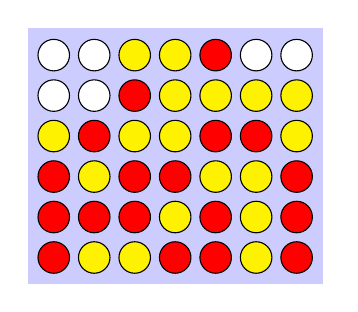
\begin{tikzpicture}%
				\fill[blue!20] (0,0) rectangle (3.75,3.25);%
				\matrix (mat) at (0,0) [matrix of nodes, ampersand replacement=\&, nodes={circle, minimum size=.4cm},%
				anchor= south west,%
				column sep={.1cm}, row sep={.1cm}] { \gy \&  \gy \&  \yw \& \yw \& \rd \&  \gy \&  \gy \&  \\%
	 \gy \&  \gy \&  \rd \&  \yw \& \yw \& \yw \& \yw \& \\%
	 \yw \& \rd \&  \yw \& \yw \& \rd \&  \rd \&  \yw \& \\%
	 \rd \&  \yw \& \rd \&  \rd \&  \yw \& \yw \& \rd \&  \\%
	 \rd \&  \rd \&  \rd \&  \yw \& \rd \&  \yw \& \rd \&  \\%
	 \rd \&  \yw \& \yw \& \rd \&  \rd \&  \yw \& \rd \&  \\%
					};%
	\end{tikzpicture}%
	\caption{As player 2}%
	\label{fig:monty}%
	\end{subfigure}%
	
	
	\end{figure}
	\begin{figure}[h]
		\centering
	
	%
	\begin{subfigure}[b]{0.4\linewidth}%
	\centering%
	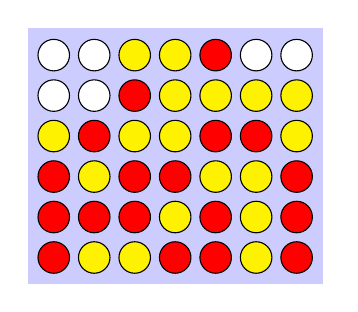
\begin{tikzpicture}%
				\fill[blue!20] (0,0) rectangle (3.75,3.25);%
				\matrix (mat) at (0,0) [matrix of nodes, ampersand replacement=\&, nodes={circle, minimum size=.4cm},%
				anchor= south west,%
				column sep={.1cm}, row sep={.1cm}] { \gy \&  \gy \&  \yw \& \yw \& \rd \&  \gy \&  \gy \&  \\%
	 \gy \&  \gy \&  \rd \&  \yw \& \yw \& \yw \& \yw \& \\%
	 \yw \& \rd \&  \yw \& \yw \& \rd \&  \rd \&  \yw \& \\%
	 \rd \&  \yw \& \rd \&  \rd \&  \yw \& \yw \& \rd \&  \\%
	 \rd \&  \rd \&  \rd \&  \yw \& \rd \&  \yw \& \rd \&  \\%
	 \rd \&  \yw \& \yw \& \rd \&  \rd \&  \yw \& \rd \&  \\%
					};%
	\end{tikzpicture}%
	\caption{As player 2}%
	\label{fig:monty}%
	\end{subfigure}%
%
\begin{subfigure}[b]{0.4\linewidth}%
	\centering%
	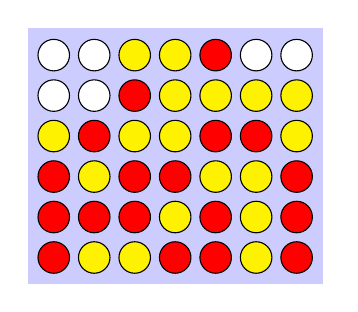
\begin{tikzpicture}%
				\fill[blue!20] (0,0) rectangle (3.75,3.25);%
				\matrix (mat) at (0,0) [matrix of nodes, ampersand replacement=\&, nodes={circle, minimum size=.4cm},%
				anchor= south west,%
				column sep={.1cm}, row sep={.1cm}] { \gy \&  \gy \&  \yw \& \yw \& \rd \&  \gy \&  \gy \&  \\%
	 \gy \&  \gy \&  \rd \&  \yw \& \yw \& \yw \& \yw \& \\%
	 \yw \& \rd \&  \yw \& \yw \& \rd \&  \rd \&  \yw \& \\%
	 \rd \&  \yw \& \rd \&  \rd \&  \yw \& \yw \& \rd \&  \\%
	 \rd \&  \rd \&  \rd \&  \yw \& \rd \&  \yw \& \rd \&  \\%
	 \rd \&  \yw \& \yw \& \rd \&  \rd \&  \yw \& \rd \&  \\%
					};%
	\end{tikzpicture}%
	\caption{As player 2}%
	\label{fig:monty}%
	\end{subfigure}%
%
	\end{figure}%
	%
	
	\newpage
	\clearpage

	\section{Successor Function}
		We perform two different types of ordering: static and dynamic. The static ordering is very simple. We initialize an array storing what we have determined to be an ordering that usually results in a cutoff. First we try the center, then the two columns around it, then the ones next to that, then the edges. This gives a decent performance boost.
		
		The dynamic ordering is done using the concept of a \emph{killer heuristic}. The basic idea is that moves at the same level of the game tree are often quite similar, and what helped us prune at one node may help prune at a sibling. This is clearly the case in connect 4. Take figure \ref{fig:2} for example. If we started our search at the board state shown in \ref{fig:1} we would arrive at this state at a depth of 3 in our search. However we could arrive at these states in multiple ways. No matter which way we use to arrive the best move choice will remain the same. By storing this best move in an array of length 42 (the number of moves possible) at index 3 we can assure that the next time we arrive at this state we will be able to immidiately find the best choice and possibly prune the rest of the search tree. Although in this early there may be other states between arriving at this state for the second time, the optimal move still tends to remain the same for similar states. For example for any placement of the second red piece except the center column, yellows best move remains the center column.
	\begin{figure}[h]
	\centering
		\begin{subfigure}[b]{0.4\textwidth}
		\centering
		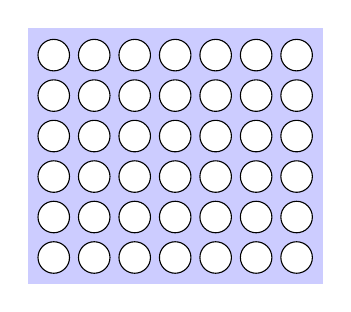
\begin{tikzpicture}
			\fill[blue!20] (0,0) rectangle (3.75,3.25);
			\matrix (mat) at (0,0) [matrix of nodes, ampersand replacement=\&, nodes={circle, minimum size=.4cm},
			anchor= south west,
			column sep={.1cm}, row sep={.1cm}] {
				\gy \& \gy \& \gy \& \gy \& \gy \& \gy \& \gy \\
				\gy \& \gy \& \gy \& \gy \& \gy \& \gy \& \gy \\
				\gy \& \gy \& \gy \& \gy \& \gy \& \gy \& \gy \\
				\gy \& \gy \& \gy \& \gy \& \gy \& \gy \& \gy \\
				\gy \& \gy \& \gy \& \gy \& \gy \& \gy \& \gy \\
				\gy \& \gy \& \gy \& \gy \& \gy \& \gy \& \gy \\
			};
		\end{tikzpicture}
		\caption{Initial state}
		\label{fig:1}
		\end{subfigure}
		\begin{subfigure}[b]{0.4\textwidth}
		\centering
		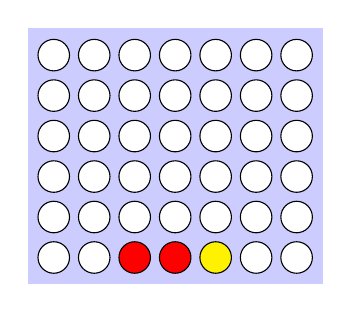
\begin{tikzpicture}
			\fill[blue!20] (0,0) rectangle (3.75,3.25);
			\matrix (mat) at (0,0) [matrix of nodes, ampersand replacement=\&, nodes={circle, minimum size=.4cm},
			anchor= south west,
			column sep={.1cm}, row sep={.1cm}] {
				\gy \& \gy \& \gy \& \gy \& \gy \& \gy \& \gy \\
				\gy \& \gy \& \gy \& \gy \& \gy \& \gy \& \gy \\
				\gy \& \gy \& \gy \& \gy \& \gy \& \gy \& \gy \\
				\gy \& \gy \& \gy \& \gy \& \gy \& \gy \& \gy \\
				\gy \& \gy \& \gy \& \gy \& \gy \& \gy \& \gy \\
				\gy \& \gy \& \rd \& \rd \& \yw \& \gy \& \gy \\
			};
		\end{tikzpicture}
		\caption{Three ply search}
		\label{fig:2}
		\end{subfigure}
	
	\end{figure}	
\end{document}